Soit $G$ un groupe, d'élément neutre $e$, et soit $E$ un ensemble.
On dit que $G$ agit sur $E$ s'il existe une application
\[
\begin{aligned}
    G \times E &\longrightarrow E \\
    (g,x) &\longmapsto g \cdot x
\end{aligned}
\]
telle que
\[
    \forall x \in E,\quad e \cdot x = x
    \qquad\text{et}\qquad
    \forall g,h \in G,\ \forall x \in E,\quad
    g \cdot (h \cdot x) = (gh) \cdot x .
\]

\begin{remarque}
    Pour tout $g \in G$, l'application
    \[
    \fonction{\varphi_g}{E}{E}{x}{g \cdot x}
    \]
    est bijective, d'inverse $\varphi_{g^{-1}}$.
\end{remarque}

\begin{proof}
    Pour tout $x \in E$,
    \[
        \varphi_g(\varphi_{g^{-1}}(x))
        = g \cdot (g^{-1} \cdot x)
        = (gg^{-1}) \cdot x
        = e \cdot x
        = x.
    \]
    De meme, $\varphi_{g^{-1}}(\varphi_g(x))=x$. Ainsi
    $\varphi_g \circ \varphi_{g^{-1}}=\operatorname{id}_E$ et
    $\varphi_{g^{-1}} \circ \varphi_g=\operatorname{id}_E$.
\end{proof}

\begin{proposition}{}{action-morphisme}
    Se donner une action de $G$ sur $E$ revient à se donner un morphisme
    de groupes
    \[
        \Phi : (G,\times) \longrightarrow (\operatorname{Bij}(E),\circ).
    \]
\end{proposition}

\begin{proof}
    Si $G$ agit sur $E$, on pose $\Phi(g)=\varphi_g$. D'apres la remarque,
    $\varphi_g$ est bien un element de $\operatorname{Bij}(E)$. De plus,
    pour tous $g,h \in G$ et tout $x \in E$,
    \[
        \varphi_g(\varphi_h(x))
        = g \cdot (h \cdot x)
        = (gh) \cdot x
        = \varphi_{gh}(x).
    \]
    Donc $\Phi(g)\circ \Phi(h)=\Phi(gh)$ : $\Phi$ est un morphisme.

    Reciproquement, soit $\Phi:G\to \operatorname{Bij}(E)$ un morphisme. On
    definit $g\cdot x=\Phi(g)(x)$. Comme $\Phi(e)=\operatorname{id}_E$, on a
    $e\cdot x=x$. Enfin, pour tous $g,h \in G$,
    \[
        g\cdot(h\cdot x)
        = \Phi(g)(\Phi(h)(x))
        = (\Phi(g)\circ\Phi(h))(x)
        = \Phi(gh)(x)
        = (gh)\cdot x.
    \]
    C'est donc une action de $G$ sur $E$.
\end{proof}

\section*{Exemples usuels}

\begin{enumerate}
    \item Si $G \subset S_n$, alors $G$ agit sur $\{1,\dots,n\}$ par
    \[
    \begin{aligned}
        G \times \{1,\dots,n\} &\longrightarrow \{1,\dots,n\} \\
        (\sigma, i) &\longmapsto \sigma(i).
    \end{aligned}
    \]
    En effet, $\operatorname{id}(i)=i$ et
    $\sigma(\tau(i))=(\sigma\circ \tau)(i)$.

    \item Tout groupe $G$ agit sur lui-meme par conjugaison :
    \[
    \begin{aligned}
        G \times G &\longrightarrow G \\
        (g, x) &\longmapsto gxg^{-1}.
    \end{aligned}
    \]
    En effet, $exe^{-1}=x$ et
    \[
        g(hxh^{-1})g^{-1}=(gh)x(gh)^{-1}.
    \]

    \item Tout groupe $G$ agit sur lui-meme par translation a gauche :
    \[
    \begin{aligned}
        G \times G &\longrightarrow G \\
        (g, x) &\longmapsto gx.
    \end{aligned}
    \]
    En effet, $ex=x$ et $g(hx)=(gh)x$.

    \item Soit $\mathbb{K}$ un corps. Le groupe $GL_n(\mathbb{K})$ agit sur
    $\mathbb{K}^n$ par
    \[
    \begin{aligned}
        GL_n(\mathbb{K}) \times \mathbb{K}^n &\longrightarrow \mathbb{K}^n \\
        (M, x) &\longmapsto Mx.
    \end{aligned}
    \]
    Cela vient de $I_nx=x$ et $M(Nx)=(MN)x$.

    Il agit aussi sur
    \[
        Gr_k(\mathbb{K}^n)
        = \{ V \subset \mathbb{K}^n \mid V \text{ est un sous-espace vectoriel de dimension } k \}
    \]
    par
    \[
    \begin{aligned}
        GL_n(\mathbb{K}) \times Gr_k(\mathbb{K}^n) &\longrightarrow Gr_k(\mathbb{K}^n) \\
        (M, V) &\longmapsto M(V).
    \end{aligned}
    \]
    En effet, une application lineaire inversible envoie un sous-espace de
    dimension $k$ sur un sous-espace de dimension $k$, puis
    $I_n(V)=V$ et $M(N(V))=(MN)(V)$.
\end{enumerate}

\section*{Orbites et stabilisateurs}

\index{Orbite}

Soit $G$ agissant sur $E$, et soit $x \in E$.
On appelle \textit{orbite} de $x$ l'ensemble
\[
    O(x)=\{g\cdot x \mid g \in G\}.
\]

\begin{proposition}{}{orbites-partition}
    Les orbites forment une partition de $E$.
\end{proposition}

\begin{proof}
    D'abord, tout element $x \in E$ appartient a son orbite, car
    $x=e\cdot x$.

    Soient ensuite $x,y \in E$. Supposons que $O(x)\cap O(y)\neq\emptyset$.
    Il existe alors $g,h\in G$ tels que $g\cdot x=h\cdot y$. On en deduit
    \[
        y = h^{-1}\cdot(g\cdot x)=(h^{-1}g)\cdot x,
    \]
    donc $y\in O(x)$. Si $z\in O(y)$, il existe $a\in G$ tel que
    $z=a\cdot y$. Comme $y=(h^{-1}g)\cdot x$, on a
    \[
        z=a\cdot((h^{-1}g)\cdot x)=(ah^{-1}g)\cdot x \in O(x).
    \]
    Ainsi $O(y)\subset O(x)$. En echangeant les roles de $x$ et $y$, on obtient
    $O(x)\subset O(y)$, donc $O(x)=O(y)$. Deux orbites sont donc soit disjointes,
    soit egales, et comme elles recouvrent $E$, elles forment une partition.
\end{proof}

On dit que l'action de $G$ sur $E$ est \textit{transitive} si
\[
    \forall x,y \in E,\quad \exists g\in G,\quad g\cdot x=y.
\]
Cela signifie exactement que $E$ est constitue d'une seule orbite.

\begin{remarque}
    La relation definie sur $E$ par
    \[
        x\sim y \iff \exists g\in G,\quad g\cdot x=y
    \]
    est une relation d'equivalence, et ses classes d'equivalence sont les orbites.
\end{remarque}

\begin{proof}
    Elle est reflexive car $x=e\cdot x$. Elle est symetrique car, si
    $y=g\cdot x$, alors $x=g^{-1}\cdot y$. Elle est transitive car, si
    $y=g\cdot x$ et $z=h\cdot y$, alors $z=(hg)\cdot x$.
    La classe de $x$ est donc exactement $O(x)$.
\end{proof}

\index{Stabilisateur}
On appelle \textit{stabilisateur} de $x$ l'ensemble
\[
    G_x=\{g\in G \mid g\cdot x=x\}.
\]

\begin{proposition}{}{stabilisateur-sous-groupe}
    Pour tout $x\in E$, $G_x$ est un sous-groupe de $G$.
\end{proposition}

\begin{proof}
    On a $e\in G_x$ car $e\cdot x=x$. Soient $g,h\in G_x$. Alors
    \[
        (gh^{-1})\cdot x
        = g\cdot(h^{-1}\cdot x).
    \]
    Or $h\cdot x=x$, donc $h^{-1}\cdot x=x$. Ainsi
    $(gh^{-1})\cdot x=g\cdot x=x$, donc $gh^{-1}\in G_x$.
    Par le critere de sous-groupe, $G_x$ est un sous-groupe de $G$.
\end{proof}

\begin{proposition}{}{stabilisateurs-conjugues}
    Si $x,y\in E$ sont dans la meme orbite et si $g\in G$ verifie
    $g\cdot x=y$, alors
    \[
        G_y=gG_xg^{-1}.
    \]
    En particulier, si $G$ est fini, alors $|G_x|=|G_y|$.
\end{proposition}

\begin{proof}
    Soit $h\in G$. On a
    \[
    \begin{aligned}
        h\in G_y
        &\iff h\cdot y=y \\
        &\iff h\cdot(g\cdot x)=g\cdot x \\
        &\iff (g^{-1}hg)\cdot x=x \\
        &\iff g^{-1}hg\in G_x \\
        &\iff h\in gG_xg^{-1}.
    \end{aligned}
    \]
    Donc $G_y=gG_xg^{-1}$. La conjugaison
    $a\mapsto gag^{-1}$ etant une bijection de $G$, les deux sous-groupes ont
    le meme cardinal lorsque $G$ est fini.
\end{proof}

\begin{theoreme}{}{orbite-stabilisateur}
    Soit $G$ agissant sur $E$, et soit $x \in E$. L'application
    \[
    \begin{aligned}
        G/G_x &\longrightarrow O(x) \\
        gG_x &\longmapsto g\cdot x
    \end{aligned}
    \]
    est bien definie et bijective.
\end{theoreme}

\begin{proof}
    Soient $g_1,g_2\in G$. On a
    \[
    \begin{aligned}
        g_1G_x=g_2G_x
        &\iff g_2^{-1}g_1\in G_x \\
        &\iff (g_2^{-1}g_1)\cdot x=x \\
        &\iff g_1\cdot x=g_2\cdot x.
    \end{aligned}
    \]
    La premiere equivalence montre que l'application ne depend pas du
    representant choisi : elle est bien definie. La derniere equivalence montre
    aussi qu'elle est injective. Enfin, si $y\in O(x)$, alors il existe
    $g\in G$ tel que $y=g\cdot x$, donc $y$ est l'image de la classe $gG_x$.
    L'application est donc surjective.
\end{proof}

\begin{corollaire}{}{formule-cardinale-orbite}
    Si $G$ est fini, alors, pour tout $x \in E$,
    \[
        |G|=|G_x|\,|O(x)|.
    \]
\end{corollaire}

\begin{proof}
    D'apres le theoreme precedent, $|O(x)|=|G/G_x|$. Comme $G$ est reunion
    disjointe des classes a gauche modulo $G_x$, toutes de cardinal $|G_x|$,
    on a $|G|=|G/G_x|\,|G_x|=|O(x)|\,|G_x|$.
\end{proof}

\section*{Application : calculs sur $\mathbb{F}_p^n$}

On note $\mathbb{F}_p=\mathbb{Z}/p\mathbb{Z}$, où $p$ est premier.

\begin{theoreme}{}{cardinal-gln}
    On a
    \[
        |GL_n(\mathbb{F}_p)|
        = \prod_{i=0}^{n-1}(p^n-p^i)
        = p^{\frac{n(n-1)}{2}}\prod_{k=1}^n(p^k-1).
    \]
\end{theoreme}

\begin{proof}
    Une matrice de $GL_n(\mathbb{F}_p)$ est exactement une matrice dont les
    colonnes $C_1,\dots,C_n$ forment une base de $\mathbb{F}_p^n$.

    Pour choisir $C_1$, on peut prendre n'importe quel vecteur non nul :
    il y a $p^n-1$ choix. Une fois $C_1,\dots,C_i$ choisis linéairement
    independants, leur espace engendré est de dimension $i$, donc contient
    $p^i$ vecteurs. Pour que $C_{i+1}$ reste independant des precedents, il
    faut et il suffit de choisir
    \[
        C_{i+1}\notin \operatorname{Vect}(C_1,\dots,C_i),
    \]
    ce qui donne $p^n-p^i$ choix. Ainsi
    \[
        |GL_n(\mathbb{F}_p)|=(p^n-1)(p^n-p)\cdots(p^n-p^{n-1})
        =\prod_{i=0}^{n-1}(p^n-p^i).
    \]
    Enfin,
    \[
        \prod_{i=0}^{n-1}(p^n-p^i)
        = \prod_{i=0}^{n-1}p^i(p^{n-i}-1)
        = p^{0+1+\cdots+(n-1)}\prod_{k=1}^n(p^k-1),
    \]
    d'ou la deuxième formule.
\end{proof}

\begin{proposition}{}{transitivite-grassmannienne}
    L'action de $GL_n(\mathbb{K})$ sur $Gr_k(\mathbb{K}^n)$ est transitive.
\end{proposition}

\begin{proof}
    Soient $V,W\in Gr_k(\mathbb{K}^n)$. Choisissons une base
    $(v_1,\dots,v_k)$ de $V$ et une base $(w_1,\dots,w_k)$ de $W$. On complète
    ces familles en deux bases de $\mathbb{K}^n$ :
    \[
        (v_1,\dots,v_k,v_{k+1},\dots,v_n)
        \quad\text{et}\quad
        (w_1,\dots,w_k,w_{k+1},\dots,w_n).
    \]
    Il existe un unique automorphisme lineaire $\phi\in GL_n(\mathbb{K})$
    envoyant chaque $v_i$ sur $w_i$. Alors $\phi(V)=W$. L'action est donc
    transitive.
\end{proof}

On prend maintenant $V=\operatorname{Vect}(e_1,\dots,e_k)\subset\mathbb{F}_p^n$.
Comme l'action est transitive, $O(V)=Gr_k(\mathbb{F}_p^n)$, donc
\[
    |GL_n(\mathbb{F}_p)|=|G_V|\,|Gr_k(\mathbb{F}_p^n)|.
\]

\begin{proposition}{}{stabilisateur-grassmannienne}
    Le stabilisateur de $V$ est l'ensemble des matrices par blocs
    \[
        G_V=
        \left\{
        \begin{pmatrix}
            A & B \\
            0 & D
        \end{pmatrix}
        \ \middle|\
        A\in GL_k(\mathbb{F}_p),\
        D\in GL_{n-k}(\mathbb{F}_p),\
        B\in M_{k,n-k}(\mathbb{F}_p)
        \right\}.
    \]
    En particulier,
    \[
        |G_V|=|GL_k(\mathbb{F}_p)|\,|GL_{n-k}(\mathbb{F}_p)|\,p^{k(n-k)}.
    \]
\end{proposition}

\begin{proof}
    Ecrivons une matrice de $M_n(\mathbb{F}_p)$ par blocs relativement a la
    decomposition
    \[
        \mathbb{F}_p^n=V\oplus \operatorname{Vect}(e_{k+1},\dots,e_n):
        \qquad
        M=
        \begin{pmatrix}
            A & B \\
            C & D
        \end{pmatrix}.
    \]
    Pour $x\in V$, les dernieres coordonnees de $Mx$ sont donnees par $Cx$.
    Ainsi $M(V)\subset V$ si et seulement si $C=0$. Comme $M$ est inversible et
    $\dim M(V)=\dim V=k$, la condition $M(V)\subset V$ equivaut alors a
    $M(V)=V$.

    Il reste donc a determiner quand une matrice triangulaire par blocs
    \[
        \begin{pmatrix}
            A & B \\
            0 & D
        \end{pmatrix}
    \]
    est inversible. Si elle est inversible, sa restriction a $V$ est un
    automorphisme de $V$, donc $A\in GL_k(\mathbb{F}_p)$. De plus, l'application
    induite sur le quotient $\mathbb{F}_p^n/V$ est un automorphisme, donc
    $D\in GL_{n-k}(\mathbb{F}_p)$. Reciproquement, si $A$ et $D$ sont
    inversibles, alors
    \[
        \begin{pmatrix}
            A & B \\
            0 & D
        \end{pmatrix}
        \begin{pmatrix}
            A^{-1} & -A^{-1}BD^{-1} \\
            0 & D^{-1}
        \end{pmatrix}
        =
        \begin{pmatrix}
            I_k & 0 \\
            0 & I_{n-k}
        \end{pmatrix},
    \]
    donc la matrice est inversible.

    Enfin, $B$ est quelconque et possede $k(n-k)$ coefficients dans
    $\mathbb{F}_p$, donc il y a $p^{k(n-k)}$ choix pour $B$.
\end{proof}

\begin{theoreme}{}{cardinal-grassmannienne}
    Le nombre de sous-espaces vectoriels de dimension $k$ de $\mathbb{F}_p^n$
    est
    \[
        |Gr_k(\mathbb{F}_p^n)|
        =
        \frac{|GL_n(\mathbb{F}_p)|}
        {|GL_k(\mathbb{F}_p)|\,|GL_{n-k}(\mathbb{F}_p)|\,p^{k(n-k)}}
        =
        \prod_{i=0}^{k-1}\frac{p^n-p^i}{p^k-p^i}.
    \]
\end{theoreme}

\begin{proof}
    La premiere formule vient du corollaire precedent, applique a l'action
    transitive de $GL_n(\mathbb{F}_p)$ sur $Gr_k(\mathbb{F}_p^n)$.

    Pour simplifier, on utilise la formule obtenue pour les groupes lineaires :
    \[
    \begin{aligned}
        |Gr_k(\mathbb{F}_p^n)|
        &=
        \frac{\prod_{i=0}^{n-1}(p^n-p^i)}
        {\left(\prod_{i=0}^{k-1}(p^k-p^i)\right)
        \left(\prod_{i=0}^{n-k-1}(p^{n-k}-p^i)\right)
        p^{k(n-k)}}.
    \end{aligned}
    \]
    Or
    \[
        \prod_{i=0}^{n-1}(p^n-p^i)
        =
        \left(\prod_{i=0}^{k-1}(p^n-p^i)\right)
        \left(\prod_{i=k}^{n-1}(p^n-p^i)\right).
    \]
    Dans le second facteur, en posant $i=k+j$,
    \[
        p^n-p^{k+j}=p^k(p^{n-k}-p^j).
    \]
    Ainsi
    \[
        \prod_{i=k}^{n-1}(p^n-p^i)
        =
        p^{k(n-k)}\prod_{j=0}^{n-k-1}(p^{n-k}-p^j).
    \]
    Ces facteurs se simplifient avec le denominateur, ce qui donne
    \[
        |Gr_k(\mathbb{F}_p^n)|
        =
        \prod_{i=0}^{k-1}\frac{p^n-p^i}{p^k-p^i}.
    \]
\end{proof}

\begin{corollaire}{}{nombre-droites-vectorielles}
    Le nombre de droites vectorielles de $\mathbb{F}_p^n$ est
    \[
        \frac{p^n-1}{p-1}.
    \]
\end{corollaire}

\begin{proof}
    Une droite vectorielle est un sous-espace de dimension $1$. On applique la
    formule precedente avec $k=1$ :
    \[
        |Gr_1(\mathbb{F}_p^n)|
        =
        \frac{p^n-1}{p-1}.
    \]
\end{proof}

Pour $n=2$ et $p=3$, on obtient donc
\[
    |Gr_1(\mathbb{F}_3^2)|=\frac{3^2-1}{3-1}=4.
\]
Les quatre droites vectorielles de $\mathbb{F}_3^2$ sont
\[
    \operatorname{Vect}(1,0),\quad
    \operatorname{Vect}(0,1),\quad
    \operatorname{Vect}(1,1),\quad
    \operatorname{Vect}(2,1).
\]

\begin{center}
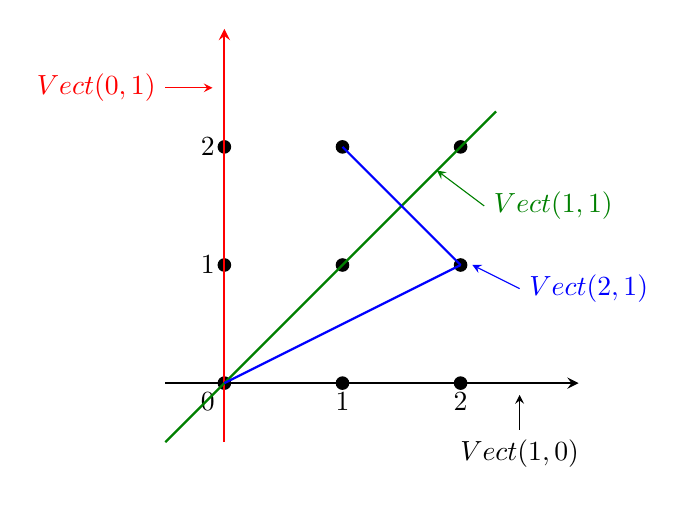
\begin{tikzpicture}[scale=1.5, >=stealth]
    \foreach \x in {0,1,2}
        \foreach \y in {0,1,2}
            \filldraw (\x,\y) circle (1.5pt);

    \node[below left] at (0,0) {0};
    \node[below] at (1,0) {1};
    \node[below] at (2,0) {2};
    \node[left] at (0,1) {1};
    \node[left] at (0,2) {2};

    \draw[->, thick] (-0.5, 0) -- (3, 0);
    \draw[<-] (2.5, -0.1) -- (2.5, -0.4) node[below] {$\operatorname{Vect}(1,0)$};

    \draw[->, thick, red] (0, -0.5) -- (0, 3);
    \draw[<-, red] (-0.1, 2.5) -- (-0.5, 2.5) node[left] {$\operatorname{Vect}(0,1)$};

    \draw[thick, green!50!black] (-0.5, -0.5) -- (2.3, 2.3);
    \draw[<-, green!50!black] (1.8, 1.8) -- (2.2, 1.5) node[right] {$\operatorname{Vect}(1,1)$};

    \draw[thick, blue] (0, 0) -- (2, 1);
    \draw[thick, blue] (1, 2) -- (2, 1);
    \draw[<-, blue] (2.1, 1) -- (2.5, 0.8) node[right] {$\operatorname{Vect}(2,1)$};
\end{tikzpicture}
\end{center}
